\chapter{Inferring Trace Links with \hfill \break a Hierarchical Bayesian Network}
\label{ch:appI-approach}

\begin{marginfigure}%[tb]
\centering

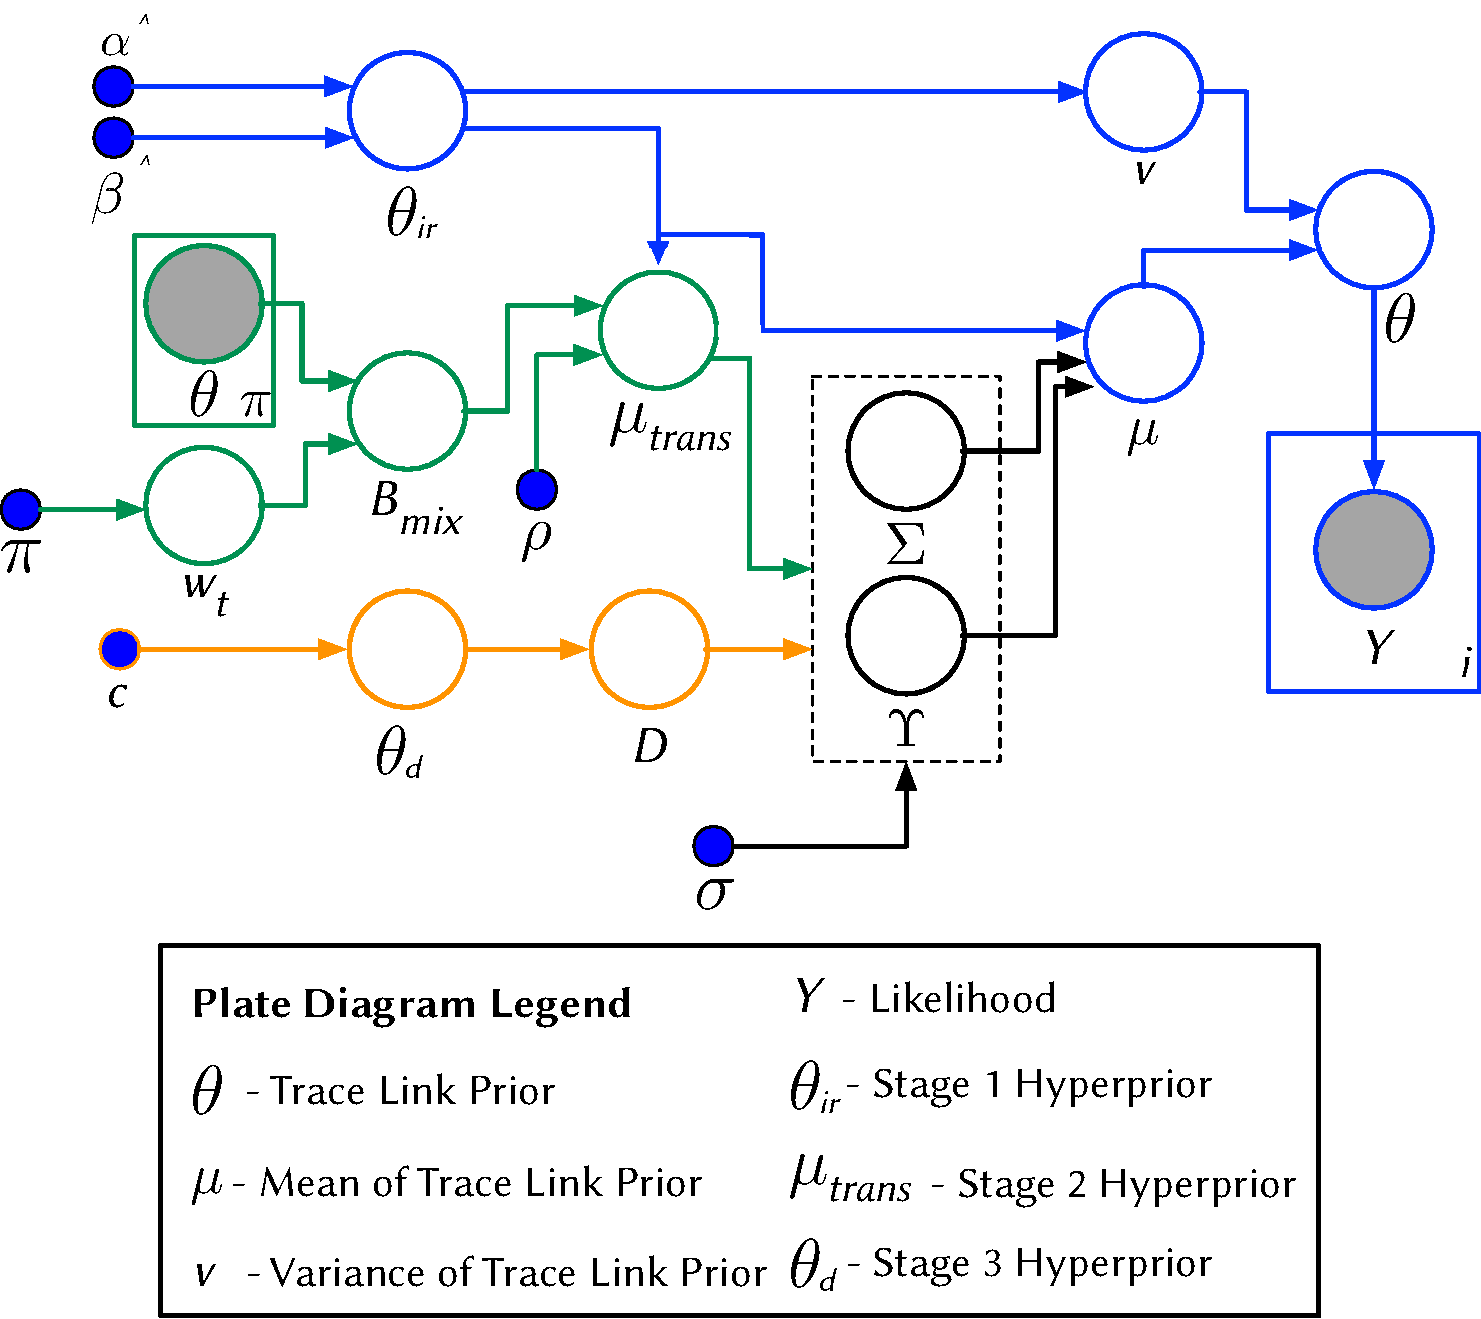
\includegraphics[width=\columnwidth]{graphics/applicationsI-approach/fig1_Model-Plate-Diagram.pdf}

\caption{Plate Diagram of \Comets HBN}
\label{fig:model-approachI}
\end{marginfigure}

In this section, we provide a formal description of \Comets probabilistic model introduced at a high level in \secref{subsec:model-motivation} \david{Check This reference}. To help aid in the comprehension of \Comets underlying model, we provide a graphical representation using plate notation~\citep{Murphy:2012} in \figref{fig:model-approachI}, which we use to guide our introduction and discussion. The model in \figref{fig:model-approachI} is computed on a \textit{per link} basis, that is between all potential links between a set of source ($S$) and target artifacts ($T$). In this section we will use $S_x$ and $T_y$ to refer to a single source and target artifact of interest respectively. \Comets probabilistic model is formally structured as an HBN, centered upon a \textit{trace link prior} $\theta$ which represents the model's prior belief about the probability that $S_x$ and $T_y$ are linked.  Our model is hierarchical, as the trace link prior is influenced by a number of \textit{hyperpriors}, which are constructed in accordance with a set of \textit{hyper-parameters} that are either derived empirically, or fixed. In \figref{fig:model-approachI}, hyperpriors are represented as empty nodes, and hyper-parameters are represented as shaded blue nodes. In general, empty nodes represent latent, or hidden, variables whereas shaded nodes represent variables that are known or empirically observed quantities. The rectangles, or ``plates'' in the diagram are used to group together variables that repeat.

To make our model easier to comprehend, we have broken it down into four major configurations, which we call \textit{stages}, indicated by different colors in \figref{fig:model-approachI}. The first stage of our model (shown in blue at top) unifies the collective knowledge of textual similarity metrics computed by IR/ML techniques. The second stage (shown in orange at the bottom) reconciles expert feedback to improve the accuracy of inferred trace links. The third stage (shown in green in the middle) accounts for transitive relationships among development artifacts, and the fourth stage combines each of the underlying stages. It should be noted that the first stage of our model can be taken as the ``base case'' upon which the other complexities build and is always required to infer the existence of a trace link.  The order of calculation starts with the first stage and proceeds sequentially. The design and parameterization of our model presented in this section is not arbitrary, but instead based on the well-founded theory of \textit{conjugate priors}~\citep{Raiffa:61} which aids in defining appropriate distributions and hyperparameters for a given prior. We center the description of our model first upon the likelihood estimation and then around the estimation of the prior probability distribution as defined by the four stages. After defining the hyperpriors for each of the four stages we briefly discuss the inference techniques we employ to estimate the posterior probability distribution of our model and thus the probability of whether a given link exists. While this section provides an overview of our model, we discuss its instantiation (including utilized IR/ML techniques) in \secref{subsec:exp-context} \david{fix the reference}.

%------------------------------------------------

\section{Estimating the Likelihood}
\label{sec:model-likelihood}

The likelihood function in our HBN models observed data so that these observations can be reconciled with our estimated prior probability distribution to infer a posterior probability.  The likelihood is shown as the observed variable $Y$ (\figref{fig:model-approachI}). The variable $i$ represents the number of observations made. In the context of traceability, we express the likelihood as a discrete Bernoulli distribution, as two artifacts can either be ``linked'' or ``not-linked'':

\begin{equation}\label{eq:likelihood}
Y = p(l_i|\theta_i)= Bern(l_i|\theta_i)
\end{equation}

\noindent \david{fix this} where $l_i$ is an observable data point ${0,1}$ for $i$ number of observations. We define an observation as a function of the textual similarity score generated by an IR technique between $S_x$ and $T_y$ and some threshold $k_i$ where any similarity above the threshold is considered an observed link, and any similarity value below this threshold is considered a non-link. The number of IR techniques or configurations utilized corresponds to the number of observations $i$.  Ideally, to capture the most accurate trace link observations from IR techniques, the threshold $k_i$ should be chosen to maximize the chance that each IR technique correctly establishes whether two artifacts are linked.  In other words, $k_i$ should be chosen for each IR technique such that the precision and recall of the technique is maximal across the entire set of considered source and target artifacts $S$ and $T$.  However, this information is not available a-priori without the consultation of a ground truth set of trace links. As we illustrate in \secref{sec:study} \david{fix this reference} this threshold can often be estimated with surprising accuracy by analyzing the distribution of similarity values an IR technique produces for a given set of artifacts. 

%-------------------------------

\section{Stage 1 - Unifying Textual Similarities between Development Artifacts}
\label{sec:model-comp1}

The first ``base'' stage of our model informs the trace link prior, represented as a probability distribution $p(\theta)$, according to the textual similarity measurements of a set of IR techniques.  However, converse to the likelihood estimation, the actual textual similarity values of IR techniques are directly used to estimate a Beta distribution (the conjugate prior of the likelihood's Bernoulli distribution). This Beta distribution is represented as follows: 

\begin{equation}\label{eq:lvl1-dist}
\theta \sim B(\mu, \nu) 
\end{equation}

\noindent where $\mu$ and $\nu$ are parameters of the Beta distribution representing its mean and variance. This prior, and its two parameters are illustrated in the right-most part of the blue segment (\figref{fig:model}). To inform this Beta distribution, the textual similarity of values of a given number $i$ of IR/ML techniques are normalized according to a sigmoid function centered upon the median of the distribution of similarity values across all $S$ and $T$ in a given dataset. Then a logistic regression is performed upon the normalized similarity values to infer the values $\hat{\alpha}$ and $\hat{\beta}$ which define a hyperprior beta distribution $\theta_{IR}$. This hyperprior with parameters are shown on the left of the blue segment (\figref{fig:model}). The mean and the variance of this hyperprior distribution then inform $\mu$ and $\nu$ of the base prior $\theta$:


\begin{equation}\label{eq:lvl1-params}
\nu = Var[\theta_{IR}] \quad \mu = Mean[\theta_{IR}]
\end{equation}

Thus, by considering the textual similarity values of a set of IR techniques, our model can effectively reconcile the collective knowledge to ultimately make an informed prediction.

%-------------------------------
\section{Stage 2 - Incorporating Developer Feedback}
\label{sec:model-comp2}

The second stage of our model is capable of leveraging human feedback by influencing the prior distribution introduced in the first stage of our model. To model expert feedback, we estimate hyperpriors $D$ and $\theta_d$, shown in orange in \figref{fig:model}. To perform this estimation, our model accepts from a developer or analyst, their confidence that a given link exists as a value between $[0,1]$. In \secref{subsec:comet-jenkins} \david{fix it} we illustrate how such feedback can be collected from developers in a lightweight manner. This confidence value serves as a parameter for estimating the distribution of the first hyperprior:

\begin{equation}
\theta_{d} \sim B(\mu_{d}=c,sd=0.01)	
\end{equation}

\noindent where $\theta_{d}$ is a Beta distribution parameterized by its mean $\mu_d$ set to the confidence value provided by a developer, and standard deviation $sd$ which we set to 0.01 signaling a low variance in the derived Beta distribution. This distribution then parameterizes the second hyperprior $D$, modeled as a Bernoulli distribution.

Now that we have derived a distribution representing developer feedback, we must define how this distribution affects the prior probability of the first stage of our model. To do this, we define reward and penalty functions $\Upsilon$ and $\Sigma$ that are influenced by $\sigma$ which represents a specified \textit{belief factor} between $[0,1]$ that controls the extent to which the feedback influences the trace link prior. The reward function is defined as $\Upsilon = \sigma*D$, whereas the penalty function is defined as $\Sigma = \sigma*(D-1)$. These factors impact the first stage prior Beta distribution by affecting its mean $\mu$:

\begin{equation}\label{eq:mean-affect}
	\mu \sim N(\mu_n= \Sigma + \Upsilon, sd=0.01)
\end{equation}

\noindent where the mean of the first stage prior is represented as a normal distribution parameterized by $\mu_n$ set to the sum of $\Sigma$ and $\Upsilon$, and a standard deviation set to 0.01. Thus, in this manner, expert feedback is utilized to influence the prior distribution that a given trace link exists. The structure of the Stage 2 hyperpriors allows \Comets HBN to effectively consider feedback from multiple developers.

%-------------------------------
\subsection{Stage 3 - Leveraging Transitive Links}
\label{sec:model-comp3}

As discussed earlier, the probability that a trace link exists between a source and target artifact can be influenced by \textit{transitive} relationships among varying software development artifacts.  The third stage of \Comets HBN is able to utilize these transitive links to improve the accuracy of its inferred trace link. However, before we describe how our model reconciles this information in a probabilistic manner, it is first important to understand the phenomena of transitive links. At a high level, a transitive link is an inherent relationship between two software artifacts ($A_1$,$A_2$) that may influence the existence of a trace link between either $A_1$ and any other artifact or $A_2$ and any other artifact. \Comet is currently capable of leveraging two types of transitive links, one based on textual-similarities (req. $\leftrightarrow$ req.) and one based on dynamic execution information (req. $\leftrightarrow$ test case). However, \Comet could also be extended to model transitive relationships between other types of artifacts, such as commit messages or issues. \figref{fig:trans-req2req} provides an illustration of both transitive link types, which we detail below. Note that for execution traces, a relationship is considered \textit{strong} between a test method and source method if the test executes the method, and \textit{weak} otherwise. For req$\leftrightarrow$req relationships, it is \textit{strong} if the textual similarity is above the threshold $\tau$, and \textit{weak} if it is below the threshold.

\begin{figure}%[tb]
\centering
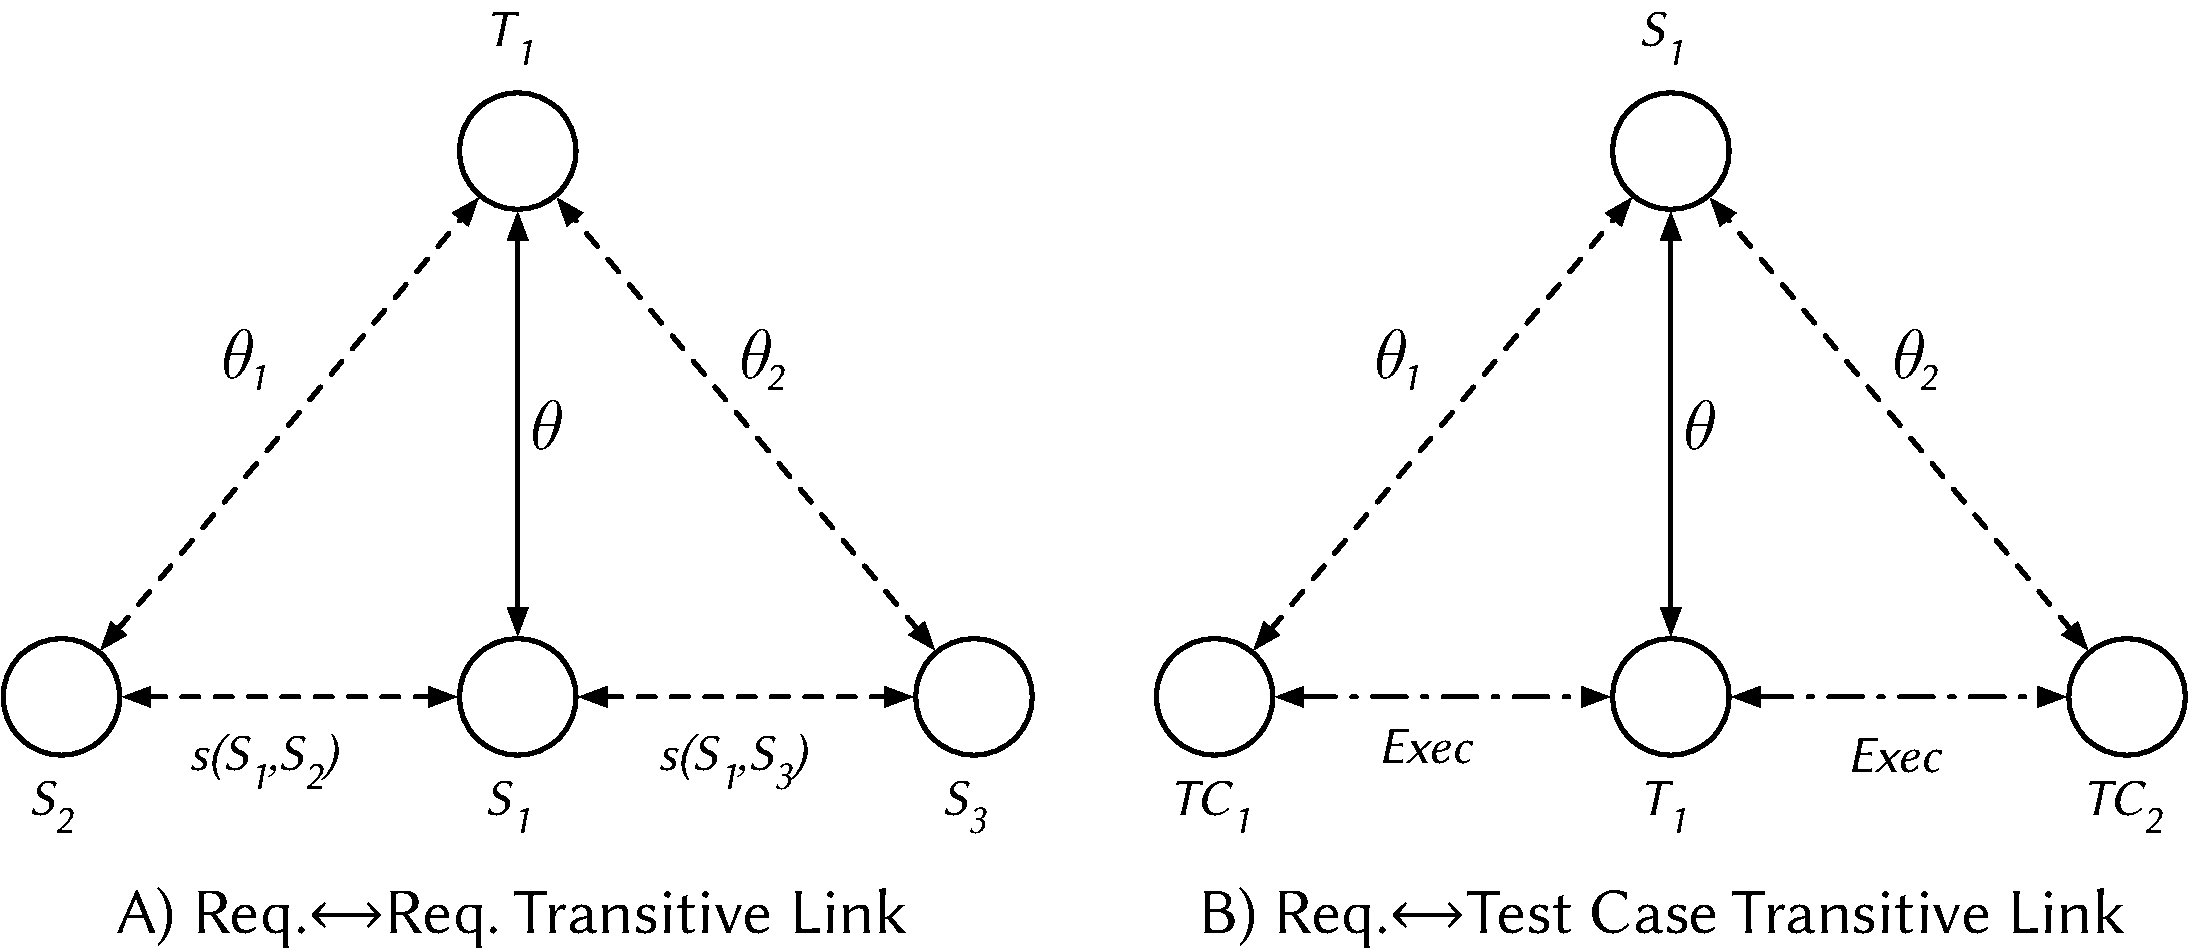
\includegraphics[width=\columnwidth]{graphics/applicationsI-approach/fig2_transitive-links.pdf}
\caption{Illustration of Transitive Links}
\label{fig:trans-req2req}
\end{figure}

\subsection{\textbf{Req. $\leftrightarrow$ Req. Links}} Consider $S_1,S_2,S_3$ as three source artifacts representing three discrete requirements documents and $T_1$ is a potential target document (\ie source code file), where the target relationship being inferred is $S_1\rightarrow T_1$, indicated by the solid line. The connections between nodes denote relationships among the artifacts. Consider the scenario in which the relationship between $S_1$ and $T_1$ is weak, but $S_1$ is highly similar to the other two requirements $S_2$ and $S_3$. Given that we know the three source artifacts are highly related, the relationships between $S_2\rightarrow T_1$ and $S_3\rightarrow T_1$ have a \textit{transitive} influence on the target relationship between $S_1$ and $T_1$. For instance, if $S_2\rightarrow T_1$ and $S_3\rightarrow T_1$ both indicate strong probabilities, then likewise the probability of the target link $S_1\rightarrow T_1$ should be increased to account for these transitive relationships.

\subsection{\textbf{Req.$\leftrightarrow$ Test Case Links}} Consider $S_1$ to be a source artifact representing a requirement document, $T_1$ to be a potential target source code file, and $TC_1,TC_2$ to be test cases, where the target relationship being inferred is $S_1\rightarrow T_1$, indicated by the solid line. Consider again the scenario in which the relationship between $S_1$ and $T_1$ is weak, whereas the relationship between $S_1$ and $TC_1,TC_2$ are stronger. If we observe that $TC_1$ and $TC_2$ are related to $T_1$ by execution information (\eg $TC_1$ and $TC_2$ both exercise $T_1$, \textit{Exec} in Fig. \ref{fig:trans-req2req}) then, this transitive relationship should influence the probability that a trace link exists between $S_1$ and $T_1$.

\subsection{\textbf{Incorporating Transitive Links into C{\footnotesize OMET}'s HBN}} In order for our HBN to incorporate transitive req. $\leftrightarrow$ req. links, it must first derive the set of requirements that are related to a given target requirement $S_x$. To accomplish this, one of several IR techniques can be used to compute textual similarity, or the first stage of our model can be used to derive the relationships, illustrated as $s(S_1,S_2)$ \& $s(S_1,S_3)$ in Fig. \ref{fig:trans-req2req}. To incorporate information from req. $\leftrightarrow$ test case links, dynamic information must be collected that provides the $Exec_1$ \& $Exec_2$ relationships illustrated in Fig. \ref{fig:trans-req2req}. In either case, a specified threshold $\tau$ signals whether a pair of requirements is related, and the total number of related requirements or test cases is specified by the hyper-parameter $\pi$.  Once the related requirements have been derived, our HBN estimates three hyperpriors, $w_t$, $B_{mix}$ and $\mu_{trans}$. First $w_t$ is formulated as a Dirichlet distribution according to the number of related transitive requirements. Then to estimate $B_{mix}$, the first stage of our HBN is computed between each related requirement and a given target artifact $T_y$. The inferred values for each transitive link, and $w_t$ are used to form a mixture model:

\begin{equation}
	B_{mix} \sim Mix(w_t,\theta_\pi)
\end{equation}

\noindent where $B_{mix}$ is a Beta mixture model parameterized by the 1st stage inference of each transitive link and $\pi$ weights modeled as a Dirichlet distribution parameterized by $\pi$. This Dirichlet distribution is then used to derive a meditated normal distribution $\mu_{trans}$:

\begin{equation}
	\mu_{trans} \sim \rho*B_{mix} + (1-\rho)*Mean[\theta_{IR}]
\end{equation}

\noindent where $Mean[\theta_{IR}]$ represents the mean of the probability distribution of IR similarity values (from stage 1) on the trace link prior and $\rho$ is represents the \textit{belief factor} of the transitive links (\eg the degree to which the transitive relationships should affect overall prior trace link probability). $\mu_{trans}$ can then be utilized to derive the reward and penalty functions introduced earlier where $\Upsilon = \sigma*(1-\mu_{trans})$ whereas $\Sigma = \sigma*\mu_{trans}$. The reward and penalty functions can then in turn be used to influence the mean of trace link prior $\mu$:

\begin{equation}\label{eq:mean-affect-combined}
	\mu \sim N(\mu_n= \mu_{trans} + \Sigma + \Upsilon, sd=0.01)
\end{equation}

\noindent in the same manner as introduced in Eq. \ref{eq:mean-affect}. In this way, our model is capable of incorporating information from transitive links, increasing the overall prior probability if transitive links are strongly connected to the target artifact $T_y$ and decreasing it if they are not strongly connected.

%-------------------------------
\section{Stage 4 - The Holistic Model}
\label{sec:model-comp4}

The holistic model combines all three underlying stages. To accomplish this, the calculations of the reward and penalty functions for affecting the mean $\mu$ of the overall prior are modified to incorporate information from both expert feedback and transitive links:

\begin{equation}
\begin{split}
	\Upsilon \sim (1-\mu_{trans})*\sigma*D \\
	\Sigma \sim \mu_{trans}*\sigma*(D-1)
\end{split}
\end{equation}

\noindent Then Eq. \ref{eq:mean-affect-combined} can be used to derive the new mean for the overall prior probability distribution of the model.

%-------------------------------
\section{Inferring the Posterior}
\label{sec:model-posterior}

In order to reason about the probability that a trace link exists, we must estimate the posterior probability distribution of our hierarchical model $p(\Theta|L)$ according to the observable data $L$ and prior knowledge of the link $p(\Theta)$. Here $p(\Theta)$ encompasses the trace link prior and all constituent hyperpriors depending upon the stage of the model.  Once the posterior has been estimated, \Comet utilizes the \textit{mean} of the distribution as the general probability that a link exists. We can represent the general calculation of the posterior for our model using using Bayes Theorem as follows:  

\vspace{-0.3cm}
\begin{equation} \label{eq_bayes}
p(\Theta|L) = \dfrac{p(\Theta)p(L|\Theta)}{\int p(\Theta)p(L|\Theta)d\Theta} \propto p(\Theta) \prod\limits_{i=1}^n p(L_i|\Theta_i)
\end{equation}

\noindent where $n$ represents the total number of observations (\ie the number of underlying IR techniques and configurations).  \Comets HBN is non-trivial, and thus the posterior $p(\Theta|L)$ cannot be computed analytically. Therefore, we turn to approximation techniques for estimating the posterior probability distribution. Comet can currently utilize three different techniques including (i) Maximum a Posteriori (MAP) estimation~\cite{Bassett2018MaximumEstimators}, a Markov Chain Monte Carlo (MCMC) technique via the No-U-Turn sampling (NUTS) process~\cite{Hoffman2011TheCarlo}, and a machine learning-based technique called Variational Inference (VI)~\cite{Bishop:2006}. We provide experimental results in Sec. \ref{sec:results} for all techniques for Stage 1 of \Comets model, and NUTS/MAP for Stages 2-4, as VI cannot be applied to more complex stages of the model.

